\documentclass[a4paper]{article}

\usepackage[english]{babel}
\usepackage[utf8]{inputenc}
\usepackage{apacite}
\usepackage{graphicx}
\usepackage{tikz}
\usetikzlibrary{positioning}
\usepackage{xcolor}
\usepackage[colorinlistoftodos]{todonotes}

\makeatletter
\def\BState{\State\hskip-\ALG@thistlm}
\makeatother

\title{Gameplay Design \\ Assignment 2 }

\author{
  Bowald, Johan\\
  \texttt{bowaldj@student.chalmers.se}
  \and
  Odbjer, Sebastian\\
  \texttt{sebastian.odbjer@gmail.com}
}

\date{\today}

\tikzset{
    vertex/.style = {
        circle,
        fill  = black,
        outer sep = 2pt,
        inner sep = 1pt,
    }
}

\begin{document}
\maketitle
\newpage

% Ricocheting Robots Game pettern analysis
\begin{figure}
\centering
  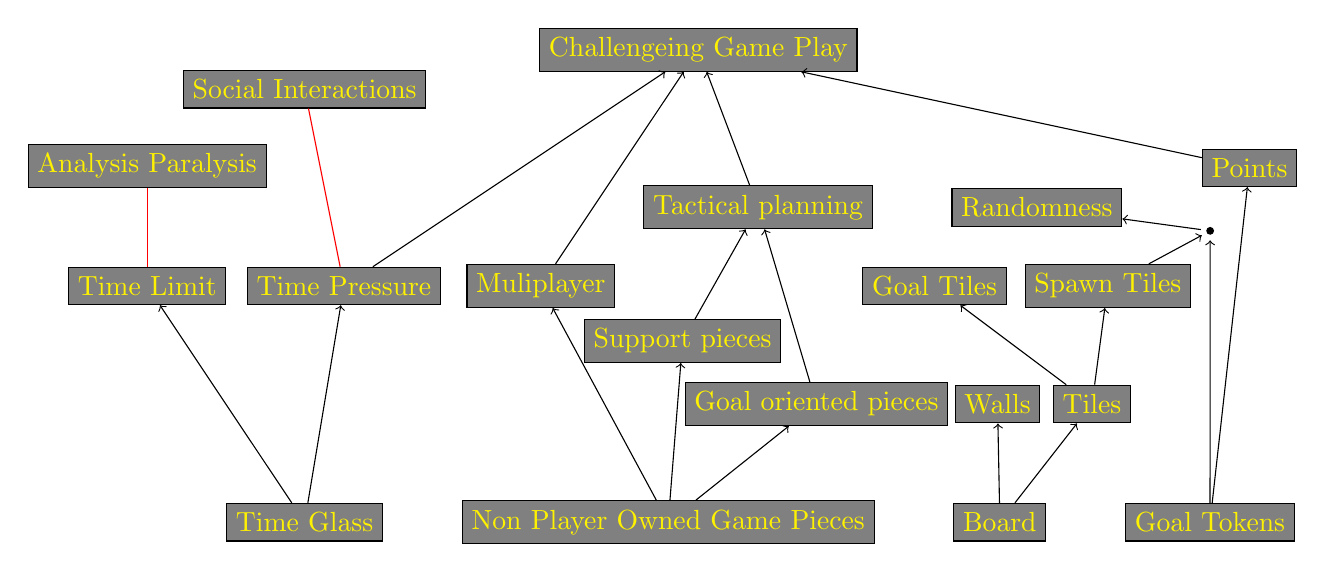
\begin{tikzpicture}
    \node[draw,fill=gray,text=yellow] (TimeGlass) at (-5,0) {Time Glass};
    \node[draw,fill=gray,text=yellow, right=of TimeGlass] (NPGP) {Non Player Owned Game Pieces};
    \node[draw,fill=gray,text=yellow, right=of NPGP] (Board) {Board};
    \node[draw,fill=gray,text=yellow, right=of Board] (GoalTokens) {Goal Tokens};

    \node[draw,fill=gray,text=yellow] at (1.5,1.5) (GoalP) {Goal oriented pieces};  
    \node[draw,fill=gray,text=yellow] at (-0.2,2.3) (SP) {Support pieces};  
    \node[draw,fill=gray,text=yellow] (Walls) at (3.8,1.5) {Walls};  
    \node[draw,fill=gray,text=yellow] (Tiles) at (5,1.5) {Tiles};  

    \node[draw,fill=gray,text=yellow] (TimeLimit) at (-7, 3) {Time Limit};  
    \node[draw,fill=gray,text=yellow] (TimeP) at (-4.5, 3) {Time Pressure};  
    \node[draw,fill=gray,text=yellow] (SI) at (-5, 5.5){Social Interactions};

    \node[draw,fill=gray,text=yellow] (MP) at (-2, 3){Muliplayer};

    \node[draw,fill=gray,text=yellow] (SpawnT) at (5.2,3) {Spawn Tiles};  
    \node[draw,fill=gray,text=yellow] (GoalT)  at (3,3) {Goal Tiles};  

    \node[draw,fill=gray,text=yellow] (Randomness) at (4.3,4){Randomness};
    \node[draw,fill=gray,text=yellow, left=of Randomness] (TacP) {Tactical planning};  
    \node[draw,fill=gray,text=yellow] (Points) at (7,4.5) {Points};
    \node[draw,fill=gray,text=yellow, above=of TimeLimit] (AP) {Analysis Paralysis};
    \node[draw,fill=gray,text=yellow] (CGP) at (0,6) {Challengeing Game Play};

    \draw node[vertex] (JointGT) at (6.5,3.7) {};

    \draw[->,draw=black] (TimeGlass) to (TimeLimit);
    \draw[->,draw=black] (TimeGlass) to (TimeP);

    \draw[->,draw=black] (NPGP) to (GoalP);
    \draw[->,draw=black] (NPGP) to (SP);
    \draw[->,draw=black] (Board) to (Walls);
    \draw[->,draw=black] (Board) to (Tiles);  

    \draw[->,draw=black] (GoalTokens) to (JointGT);
    \draw[->,draw=black] (SpawnT) to (JointGT);
    \draw[->,draw=black] (GoalTokens) to (Points);
    \draw[->,draw=black] (JointGT) to (Randomness);

    \draw[->,draw=black] (Tiles) to (SpawnT);
    \draw[->,draw=black] (Tiles) to (GoalT);
    \draw[->,draw=black] (NPGP) to (MP);
    \draw[->,draw=black] (MP) to (CGP);
    \draw[->,draw=black] (TimeP) to (CGP);
    \draw[->,draw=black] (Points) to (CGP);
    \draw[->,draw=black] (TacP) to (CGP);
    \draw[->,draw=black] (SP) to (TacP);
    \draw[->,draw=black] (GoalP) to (TacP);


    \draw[-,draw=red] (TimeLimit) to (AP);
    \draw[-,draw=red] (TimeP) to (SI);

  \end{tikzpicture}

  \caption{Analysis of Richocheting Robots using Game Design Pattern} 
  \label{fig:RRW}
\end{figure}

\begin{figure}

\centering
  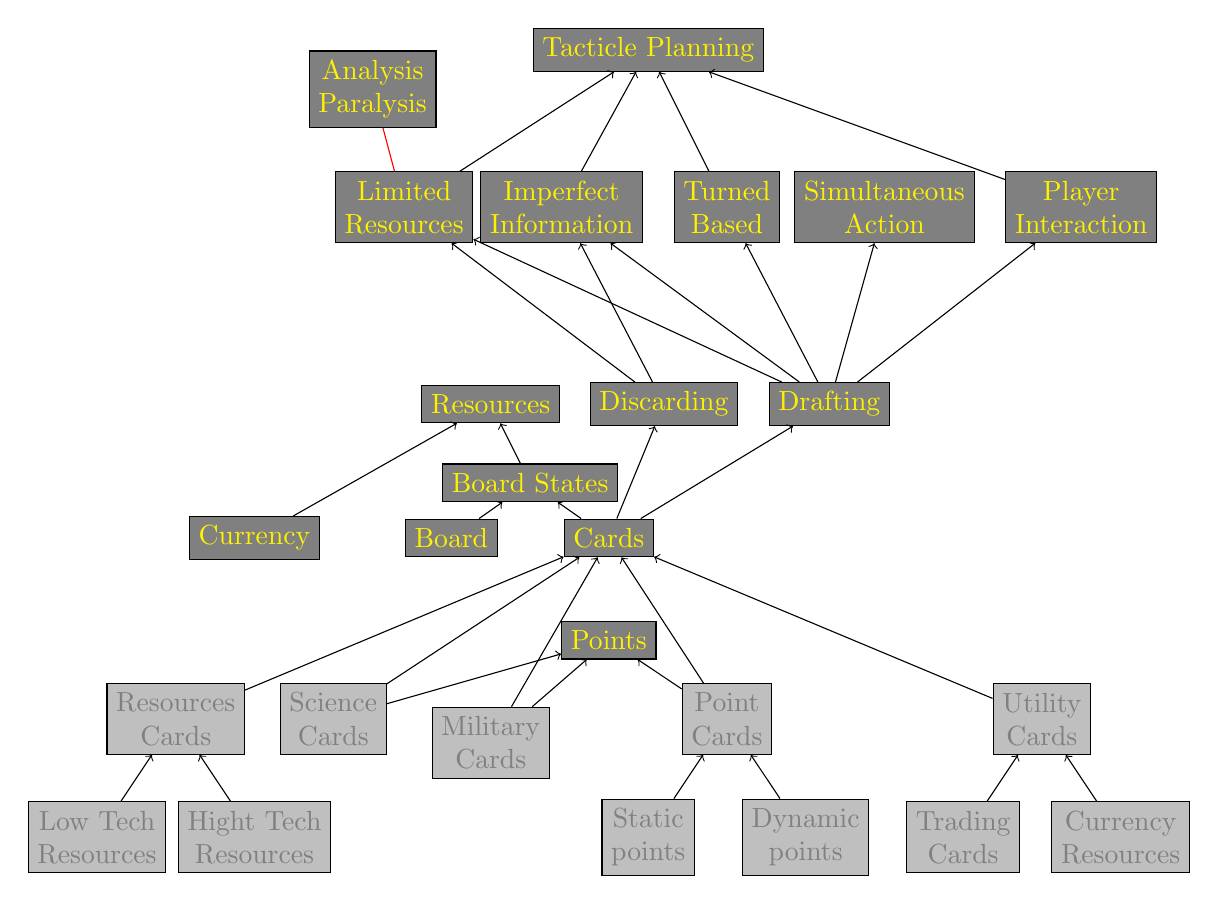
\begin{tikzpicture}

  \node[draw,fill=gray!50,text=gray, align=center] (LTRe) at (-6,0) {Low Tech\\ Resources};
  \node[draw,fill=gray!50,text=gray, align=center] (HTRe) at (-4,0){Hight Tech\\ Resources};

  \node[draw,fill=gray!50,text=gray, align=center] (CuRe) at (7,0) {Currency \\Resources};
  \node[draw,fill=gray!50,text=gray, align=center] (TrCa) at (5,0) {Trading \\Cards};  

  \node[draw,fill=gray!50,text=gray, align=center] (StPo) at (1,0) {Static\\points};
  \node[draw,fill=gray!50,text=gray, align=center] (DyPo) at (3,0) {Dynamic\\points};
  
  \node[draw,fill=gray!50,text=gray, align=center] (ReCa) at (-5,1.5) {Resources\\ Cards};
  \draw[->,draw=black] (LTRe) to (ReCa);
  \draw[->,draw=black] (HTRe) to (ReCa);
  \node[draw,fill=gray!50,text=gray, align=center] (ScCa) at (-3,1.5) {Science\\Cards};
  \node[draw,fill=gray!50,text=gray, align=center] (MiCa) at (-1,1.2) {Military\\Cards};
  \node[draw,fill=gray!50,text=gray, align=center] (PoCa) at (2,1.5) {Point\\Cards};
  \draw[->,draw=black] (DyPo) to (PoCa);
  \draw[->,draw=black] (StPo) to (PoCa);
  \node[draw,fill=gray!50,text=gray, align=center] (UtCa) at (6,1.5) {Utility\\Cards};
  \draw[->,draw=black] (TrCa) to (UtCa);
  \draw[->,draw=black] (CuRe) to (UtCa);

  \node[draw,fill=gray,text=yellow] (Po) at (0.5,2.5) {Points};

  \draw[->,draw=black] (ScCa) to (Po);
  \draw[->,draw=black] (MiCa) to (Po);
  \draw[->,draw=black] (PoCa) to (Po);

  \node[draw,fill=gray,text=yellow] (Ca) at (0.5,3.8) {Cards};

  \draw[->,draw=black] (ScCa) to (Ca);
  \draw[->,draw=black] (MiCa) to (Ca);
  \draw[->,draw=black] (PoCa) to (Ca);
  \draw[->,draw=black] (ReCa) to (Ca);
  \draw[->,draw=black] (UtCa) to (Ca);
  
  % \node[draw,fill=gray!50,text=gray, align=center ](PoTo) {Point\\Tokens};
  \node[draw,fill=gray,text=yellow] (Cu) at (-4,3.8){Currency};
  \node[draw,fill=gray,text=yellow] (Bo) at (-1.5,3.8){Board};


  % %to points, resouces
  \node[draw,fill=gray,text=yellow] (BoSt) at (-0.5,4.5) {Board States};
  \draw[->,draw=black] (Bo) to (BoSt);
  \draw[->,draw=black] (Ca) to (BoSt);

  \node[draw,fill=gray,text=yellow] (Re) at (-1,5.5) {Resources};
  \node[draw,fill=gray,text=yellow] (Di) at (1.2,5.5) {Discarding};
  \node[draw,fill=gray,text=yellow] (Da) at (3.3,5.5) {Drafting};
  \draw[->,draw=black] (Cu) to (Re);
  \draw[->,draw=black] (BoSt) to (Re);
  \draw[->,draw=black] (Ca) to (Da);
  \draw[->,draw=black] (Ca) to (Di);

  % %Drafting, discarding
  \node[draw,fill=gray,text=yellow, align=center] (ImIn) at (-0.1,8) {Imperfect\\Information};
  \node[draw,fill=gray,text=yellow, align=center] (LiRe) at (-2.1,8) {Limited\\Resources};
  \node[draw,fill=gray,text=yellow, align=center] (TuBa) at (2,8) {Turned\\Based};
  \node[draw,fill=gray,text=yellow, align=center] (SiAc) at (4,8) {Simultaneous\\Action};
  \node[draw,fill=gray,text=yellow, align=center] (PlIn) at (6.5,8) {Player\\Interaction};

  \draw[->,draw=black] (Di) to (ImIn);
  \draw[->,draw=black] (Di) to (LiRe);

  \draw[->,draw=black] (Da) to (ImIn);
  \draw[->,draw=black] (Da) to (LiRe);
  \draw[->,draw=black] (Da) to (TuBa);
  \draw[->,draw=black] (Da) to (SiAc);
  \draw[->,draw=black] (Da) to (PlIn);

  % %Drafting trading cards
  
  \node[draw,fill=gray,text=yellow, align=center] (AnPa) at (-2.5,9.5){Analysis\\Paralysis};
  \draw[-,draw=red] (LiRe) to (AnPa);
  \node[draw,fill=gray,text=yellow] (TaPl) at (1,10){Tacticle Planning};
  \draw[->,draw=black] (ImIn) to (TaPl);
  \draw[->,draw=black] (LiRe) to (TaPl);
  \draw[->,draw=black] (TuBa) to (TaPl);
  \draw[->,draw=black] (PlIn) to (TaPl);

  % \node[draw,fill=gray,text=yellow] (KiMa) {King Maker};

  \end{tikzpicture}
\caption{Analysis of 7 Wonders using Game Design Pattern}
\label{fig:A7W}
\end{figure}

\newpage
\bibliographystyle{apacite}
\bibliography{bib}

\end{document} 

